\documentclass{article}

\usepackage{graphicx}
\usepackage[hidelinks]{hyperref}
\usepackage[a4paper, total={6in, 8in}]{geometry}
\usepackage[slovak]{babel}
\usepackage{caption}
\usepackage{subcaption}

\graphicspath{./include/}

\renewcommand{\figurename}{Obr.}
\renewcommand{\contentsname}{Obsah}

\begin{document}

\begin{titlepage}
	\null\vfill

	\begin{center}
		{\Huge Regulácia výšky hladiny }
		\vskip 2cm

		{\Large Cvičenie č. 10}
		\vskip 0.5cm

		{\large Spojité procesy}
	\end{center}

	\vfill
	\vfill

	\begin{flushright}
		Filip Lobpreis \\
		Matúš Machata \\
		\small\today\\
	\end{flushright}
	\hfill
\end{titlepage}

\thispagestyle{empty}
\clearpage

\tableofcontents
\thispagestyle{empty}
\clearpage

\section{Zadanie}
\label{sec:zadanie}
\pagenumbering{arabic}

\begin{figure}[!htbp]
	\begin{center}
		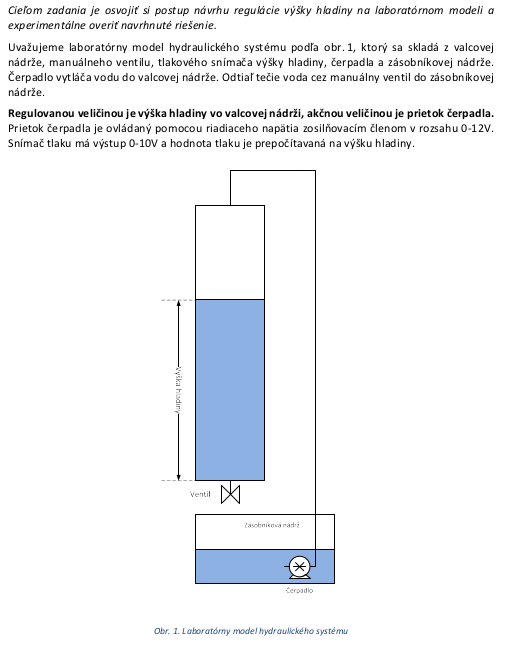
\includegraphics[width=0.8\textwidth]{./include/zadaniep1.png}
	\end{center}
	\caption{Prvá časť zadania z~cvičenia č. 9 z~predmetu spojité procesy}
	\label{fig:zadanie1}
\end{figure}

\begin{figure}[!htbp]
	\begin{center}
		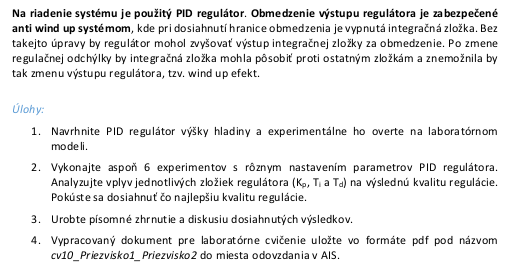
\includegraphics[width=0.8\textwidth]{./include/zadaniep2.png}
	\end{center}
	\caption{Druhá časť zadania z~cvičenia č. 9 z~predmetu spojité procesy}
		\label{fig:zadanie2}
\end{figure}

\clearpage

\section{Teória}
\label{sec:teoria}

V~tomto zadaní je našou úlohou experimentálne overiť návrh regulácie výšky hladiny na~laboratórnom
modeli hydraulického systému a~overiť navrhované riešenie. Pri~tomto zadaní sme použili už~preddefinovanú schému
v~programe \textit{Simulink} (Obr.~\ref{fig:schema}).

\begin{figure}[!htbp]
	\begin{center}
		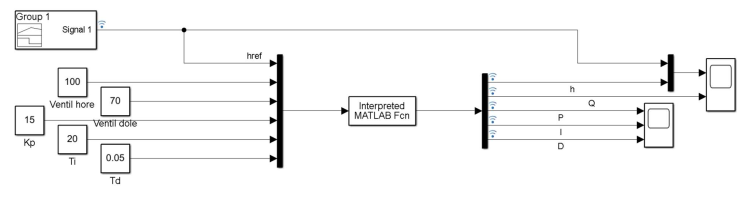
\includegraphics[width=0.8\textwidth]{./include/schema.png}
	\end{center}
	\caption{Schéma modelu z~cvičenia č. 9 z~predmetu spojité procesy}
	\label{fig:schema}
\end{figure}

V~tomto zapojení vidíme viacero vstupných signálov, tie sú už~preddefinované. \textbf{href} referenčná respektíve
žiadaná hodnota výšky hladiny. \textbf{Ventil hore} reprezentuje hodnotu vstupného prietoku do nádrže, jeho hodnoty
sú zadávané v percentách. \textbf{Ventil dole}, tato hodnota reprezentuje prietok výstupného prietoku nádrže.
Rovnako ako vstupný prietok je zadávaný v percentách. Hodnoty, ktoré sa budú meniť v priebehu meraní sú parametre
\textit{PID} regulátora.

$$ G_R(s) = K_P \left( 1 + \frac{1}{T_is} + T_ds \right) $$

Proporcionálna zložka \textbf{P} regulátora je rovná zložke $K_P$, Integračná zložka \textbf{I} je počítaná vzťahom
$\frac{K_P}{T_i}$, posledná derivačná zložka \textbf{D} regulátora je rovná $K_P T_d [-]$.
Vyššie spomenutý vzťah môžeme teda prepísať do tvaru:

$$ G_R(s) = P  + \frac{1}{s}I + Ds $$

\clearpage

\subsection{Úvod do priebehu simulácie}
\label{subsec:priebehSimulacie}

Počas priebehu simulácie sa spomínaná žiadaná hodnota výšky hladiny mení. Priebeh zmien tejto veličiny je znázornený
na obrázku Obr.~\ref{fig:ziadanaHodnota}. Hodnota žiadanej hodnoty postupne skokovo rastie po hodnotu 70 cm. Prvá
žiadaná hodnota je nastavená na 10cm čas tejto časti simulácie je nastavený na 90 sekúnd. Druha žiadaná hodnota
je nastavená na 30cm a jej čas na ustálenie hodnoty je 100 sekúnd. Každá ďalšia žiadaná hodnota výšky hladiny
je rozdelená po 20cm segmentoch a doba počas ktorej sa má hodnota ustáliť je nastavená na 100 sekúnd. Po dosiahnutí
najvyššej žiadanej hodnoty sa začne nádrž pomaly vypúšťať. Prvá časť je vypustenie nádrže na výsku hladiny 40 cm.
Čas vypúšťania na túto hodnotu je nastavený taktiež na 100 sekúnd. Druha časť vypúšťania trvá taktiež 100 sekúnd
a hodnota výšky hladiny je nastavená na 20 cm. V poslednej časti sa má nádrž úplne vypustiť. Koniec simulácie nastáva
20 sekúnd po nastavení nulovej žiadanej hodnoty hladiny nádrže.

\begin{figure}[!htbp]
	\begin{center}
		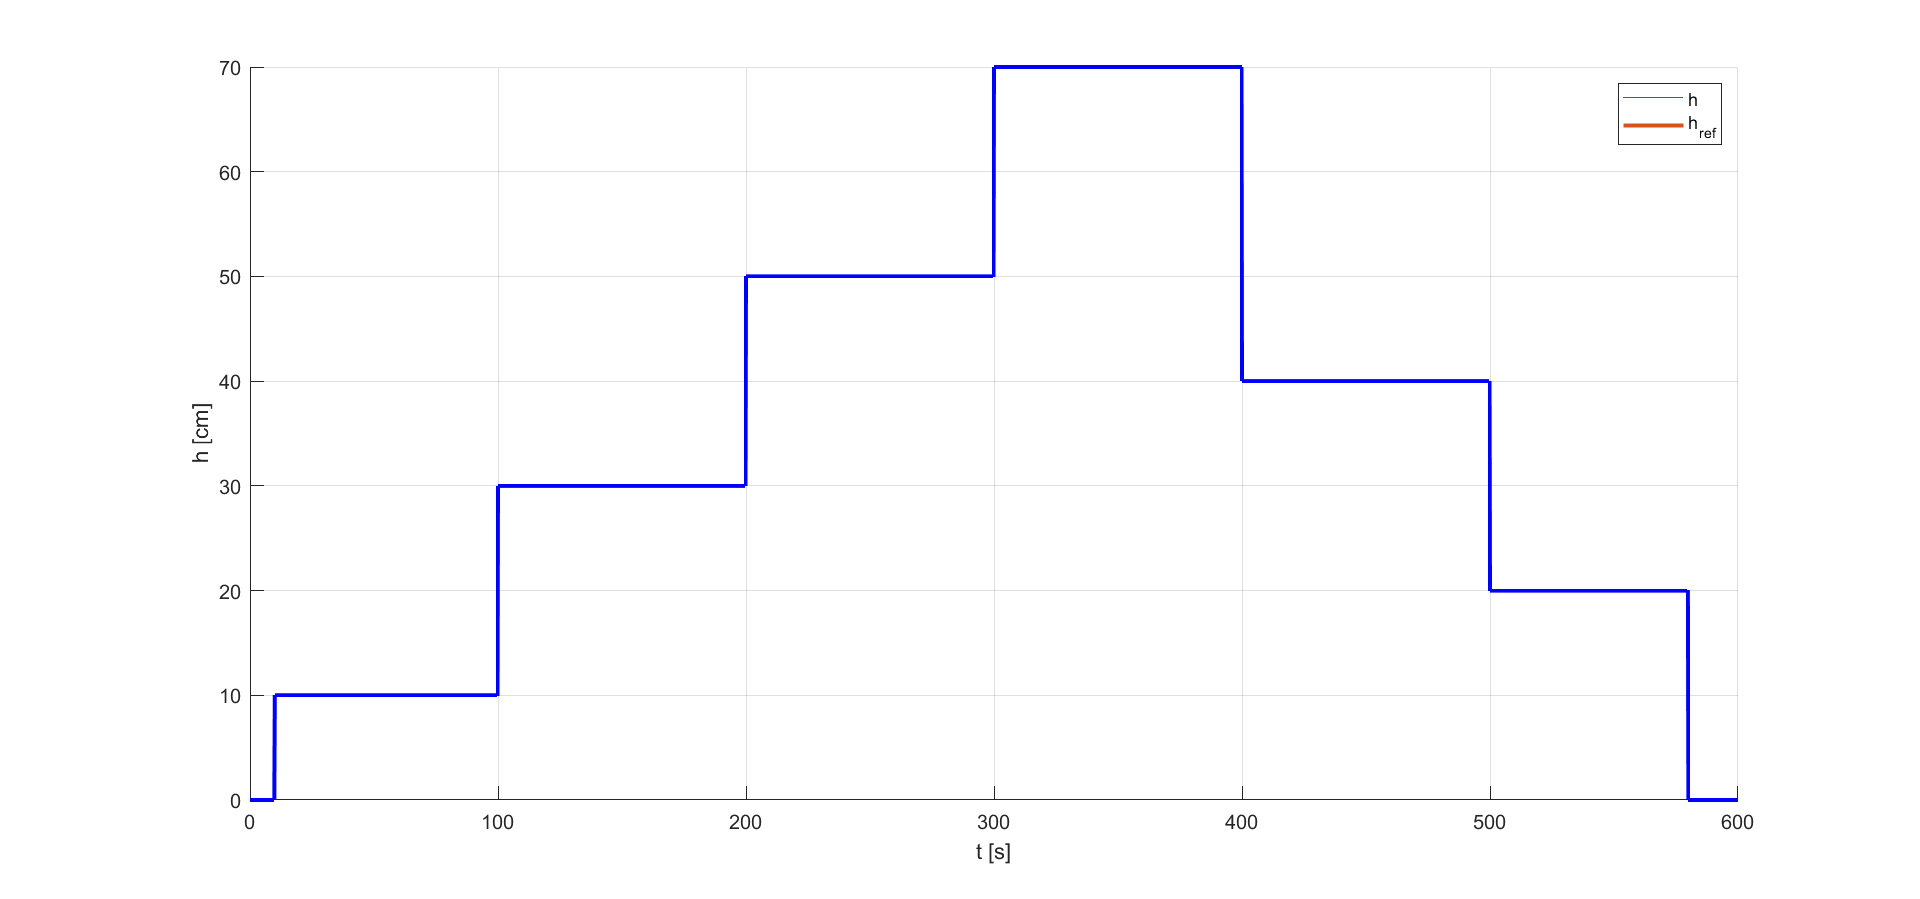
\includegraphics[width=\textwidth]{./include/ziadana_hodnota.png}
		\caption{Priebeh referenčnej teploty v~priebehu 600 sekúnd.}
		\label{fig:ziadanaHodnota}
	\end{center}
	\hfill
\end{figure}

\newpage

\section{Merania}
\label{sec:merania}

\subsection{Meranie 1}
\label{sec:meranie1}

V~prvom zadaní sme zvolili prednastavené hodnoty parametrov regulátora. Tie sú zo zadania nastavené nasledovne:

\begin{center}
\begin{tabular}{ |c|c| }
 \hline
 $K_p [-]$ & 15 \\
 $T_i [-]$ & 20 \\
 $T_d [-]$ & 0,05 \\
 \hline
\end{tabular}
\end{center}

Výsledok simulácie môžeme vidieť na~obrázku Obr.~\ref{fig:m1}.

\begin{figure}[!htbp]
	\begin{center}
		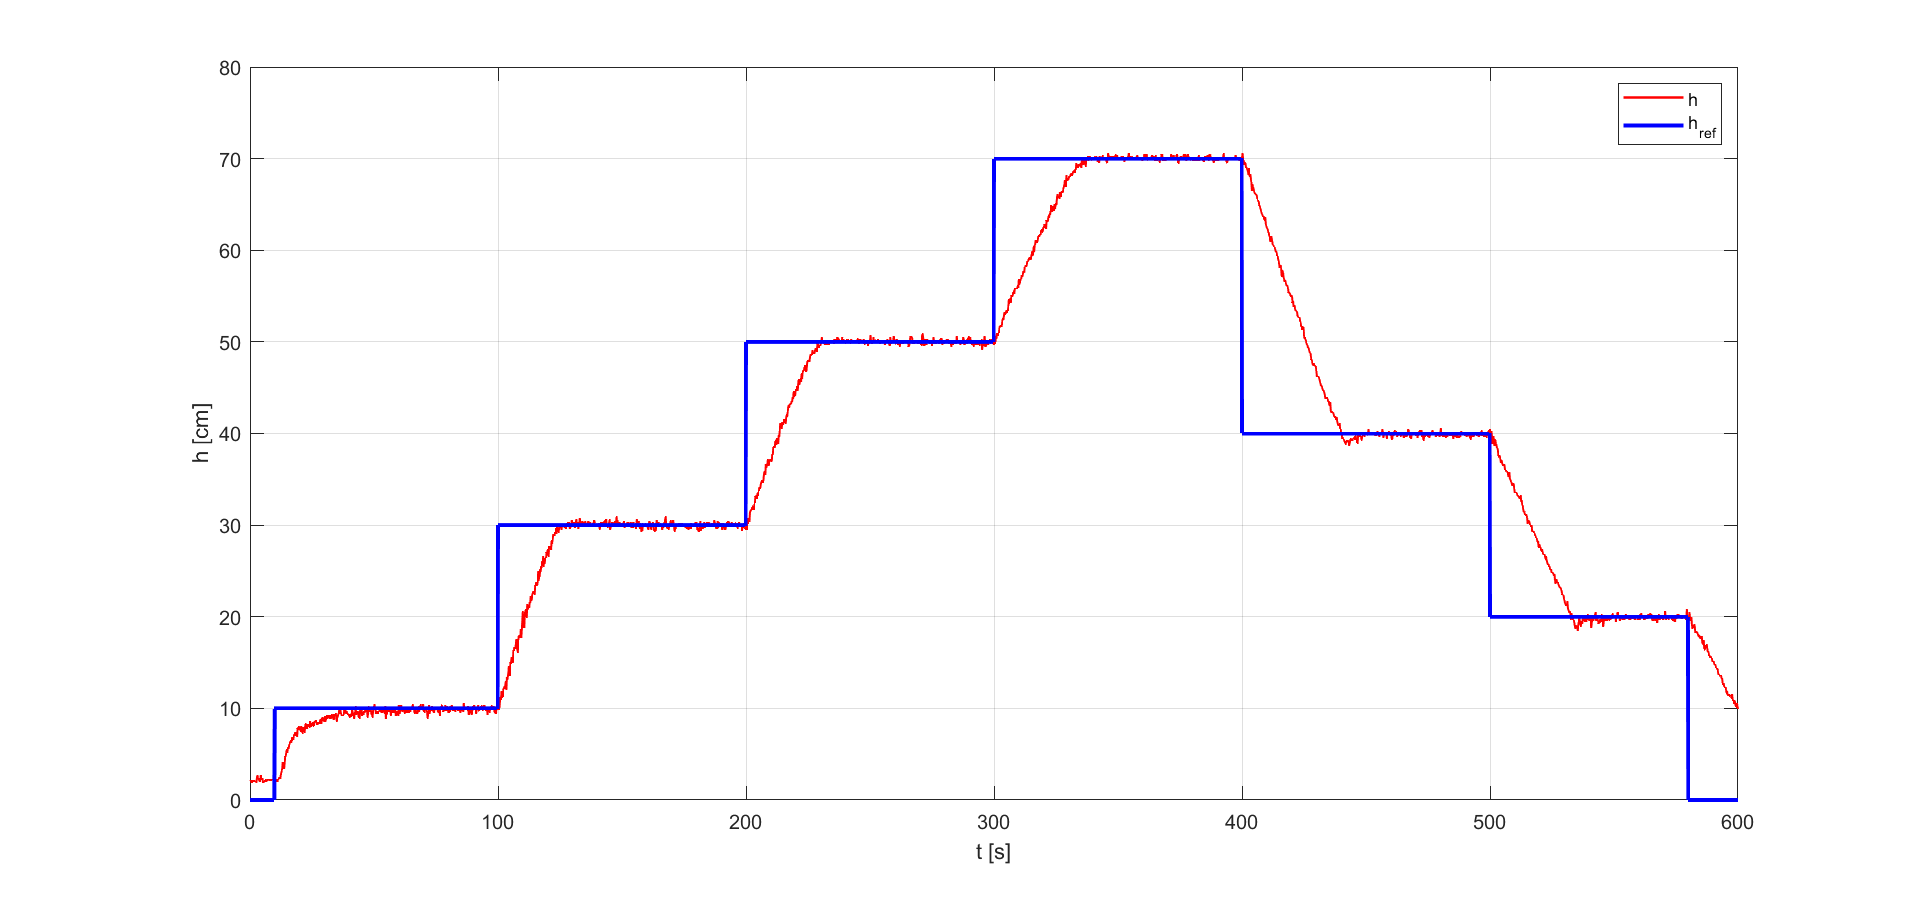
\includegraphics[width=\textwidth]{./include/meranie1.png}
	\end{center}
	\caption{Graf žiadanej a~meranej hodnoty výšky hladiny na~snímači v~prvom meraní [cm].}
	\label{fig:m1}
\end{figure}

Toto nastavenie regulátorov ovplyvnilo okolie, v ktorom sme nastavovali hodnoty v ďalších meraniach. Po zistení
priebehu výstupného signálu zobrazeného na Obr.~\ref{fig:m1} sme sa snažili dosiahnuť čo najrýchlejšiu reguláciu
výstupného signálu zo systému. Na dosiahnutie tohto cieľu sme zväčšili derivačnú zložku regulátora.
Tá zabezpečuje najrýchlejšiu odpoveď regulátora na zmenu výstupného signálu. Táto zložka zároveň zavádza šum
do akčného zásahu systému. Ďalšia zložka, ktorá zabezpečuje postupný rast akčného zásahu systému je integračná
zložka. Tá sa skladá ako bolo spomenutý v sekcii~\ref{sec:teoria} z parametrov $K_p$ a $T_i$. Pričom táto zložka
priamo úmerne závisí od zložky $K_p$ a nepriamo od $T_i$. Zmenu, ktorú sme vykonali bola zmena parametru
zosilnenia regulátora $K_p$.

\clearpage

\subsection{Meranie 2}
\label{sec:meranie2}

V druhom meraní sme si zvolili hodnoty:
Výsledok simulácie môžeme vidieť na obrázku Obr.~\ref{fig:m1}.

\begin{center}
\begin{tabular}{ |c|c| }
 \hline
 $K_p [-]$ & 30 \\
 $T_i [-]$ & 20 \\
 $T_d [-]$ & 0,1 \\
 \hline
\end{tabular}
\end{center}

\begin{figure}[!htbp]
	\begin{center}
		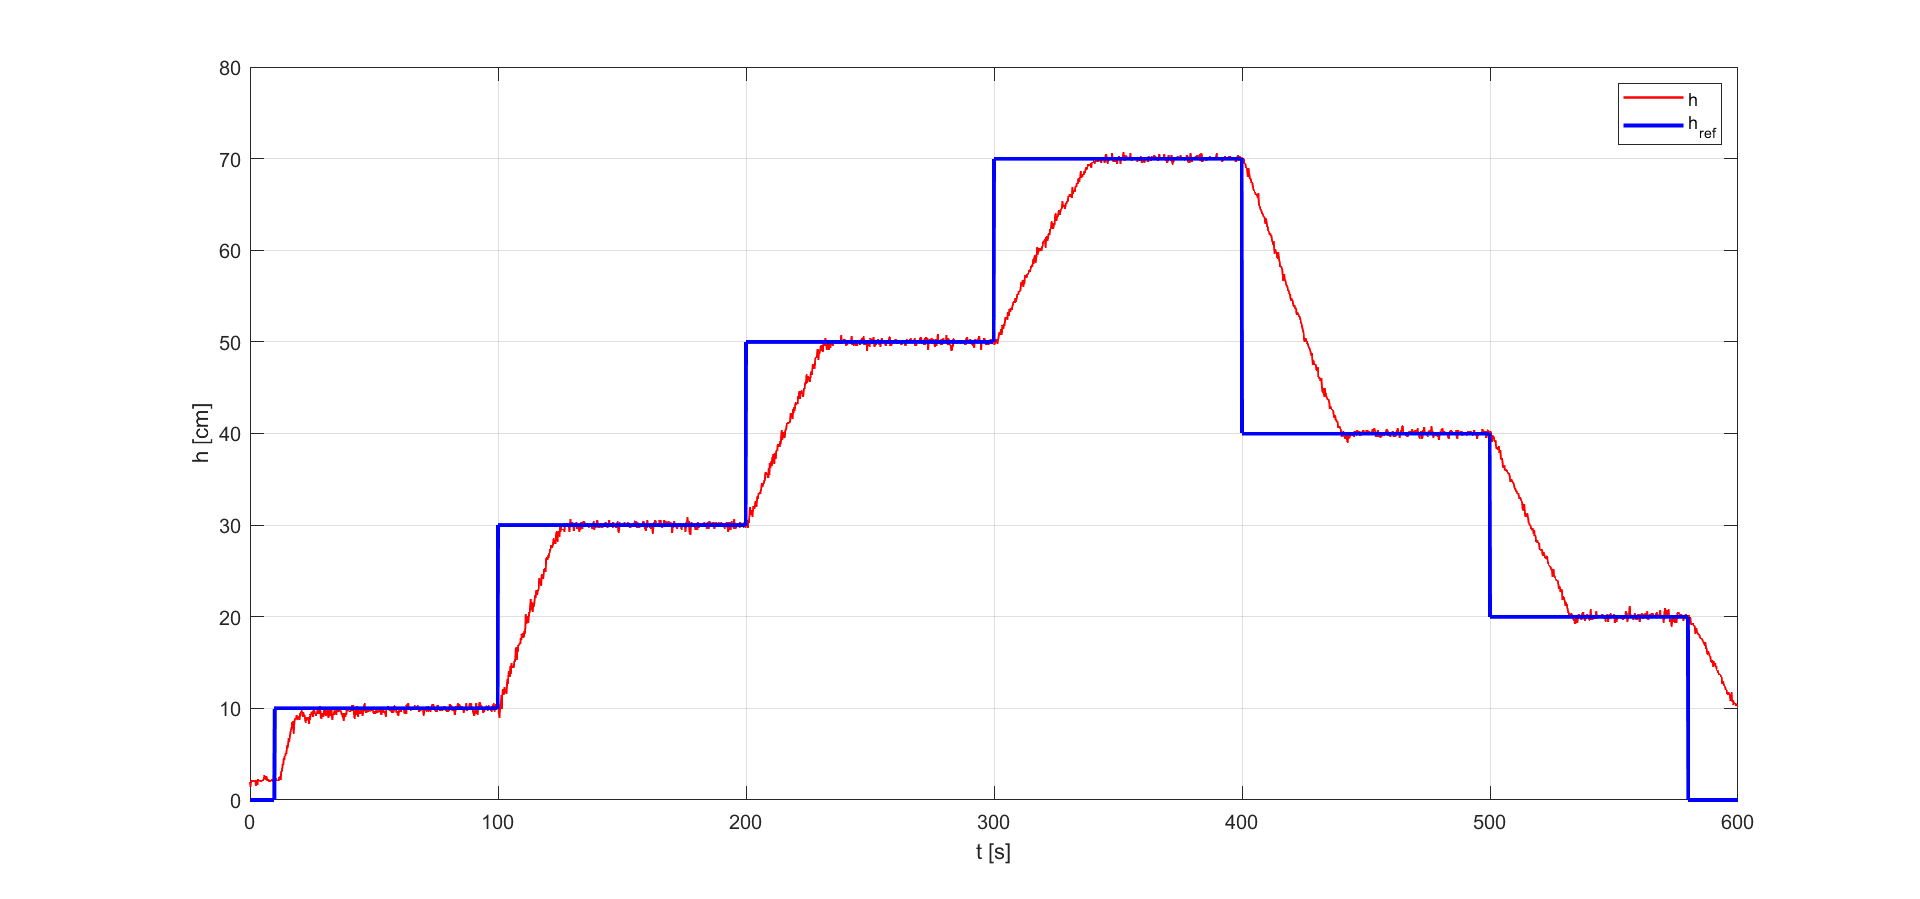
\includegraphics[width=\textwidth]{./include/meranie2.png}
	\end{center}
	\caption{Graf žiadanej a~meranej hodnoty výšky hladiny na~snímači v~druhom meraní [cm].}
	\label{fig:m2}
\end{figure}

Pri druhom meraní sme si zmenili parametre regulátora. V porovnaní s prvým meraním si môžeme všimnúť,
že preregulovanie pri vypúšťaní nádrže nebolo také viditeľné. Zároveň nábeh výšky vodného stĺpca v nádrži
z 0cm na 10cm bol rýchlejší. Tieto výhody prišli aj s jednou nevýhodou. Zašumenie výstupného signálu
systému (výšky hladiny) bolo viditeľnejšie.

\clearpage

\subsection{Meranie 3}
\label{sec:meranie3}

V treťom meraní sme si zvolili hodnoty: 
Výsledok simulácie môžeme vidieť na obrázku Obr.\ref{fig:m3}.

\begin{center}
\begin{tabular}{ |c|c| }
 \hline
 $K_p [-]$ & 50 \\
 $T_i [-]$ & 20 \\
 $T_d [-]$ & 0,5 \\
 \hline
\end{tabular}
\end{center}


\begin{figure}[!htbp]
	\begin{center}
		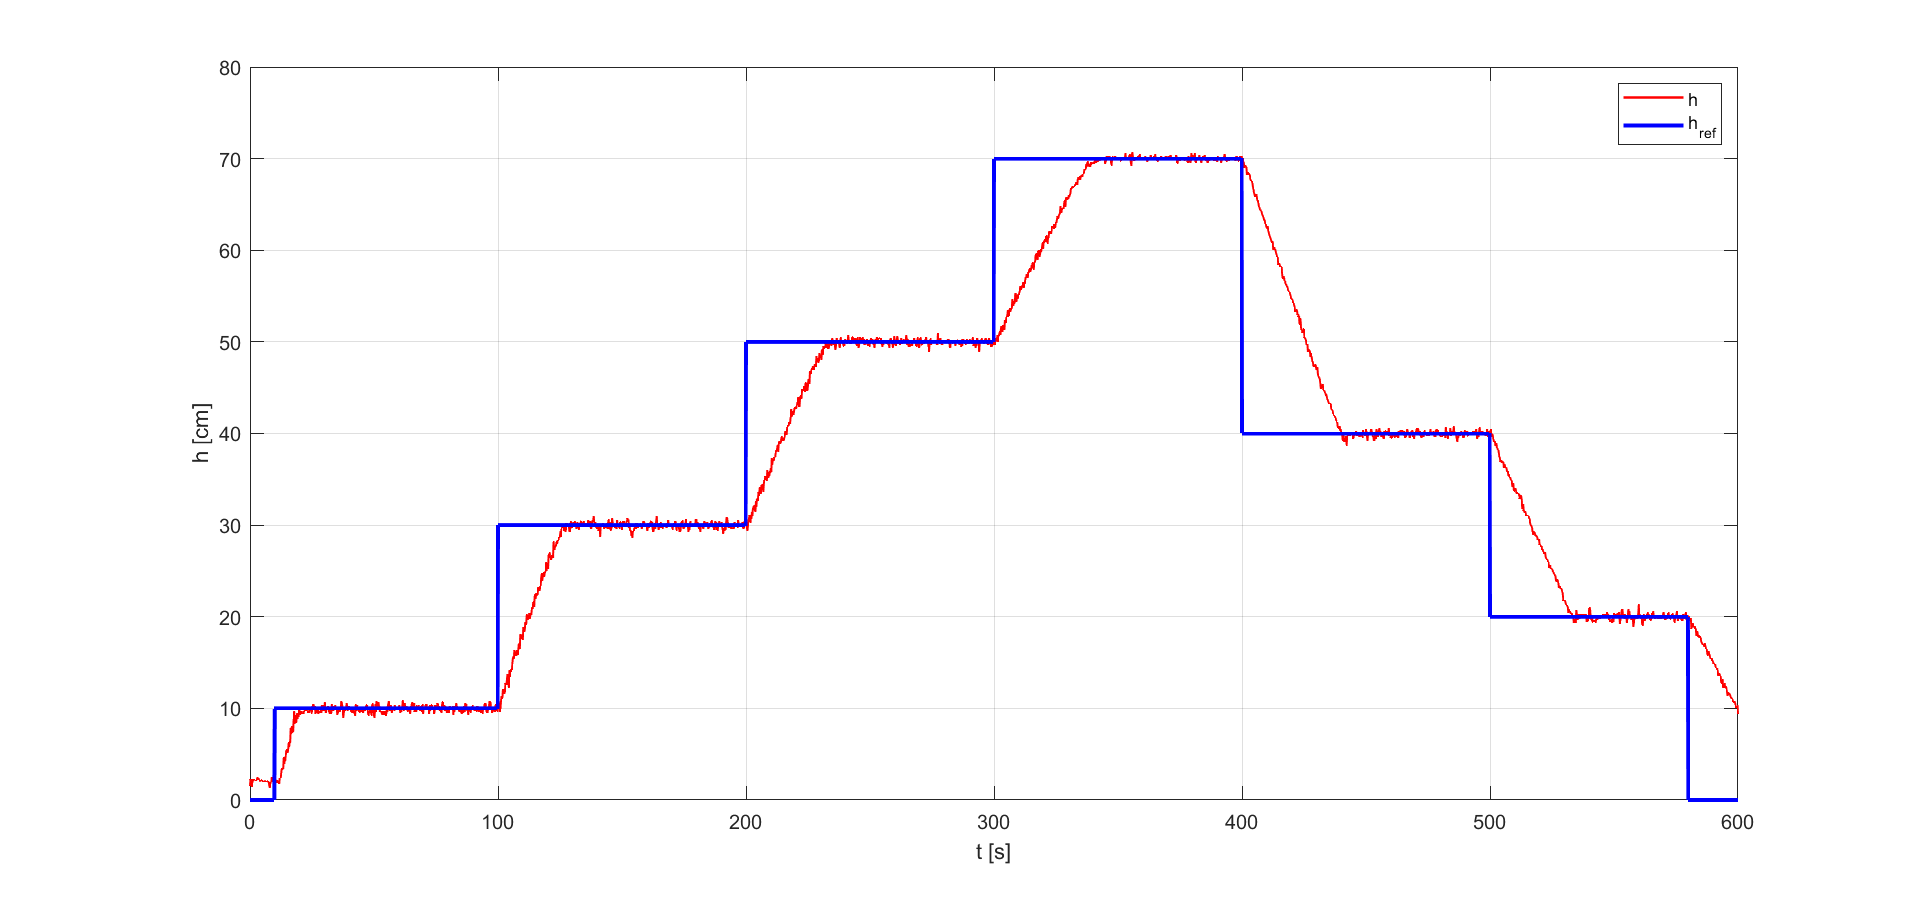
\includegraphics[width=\textwidth]{./include/meranie3.png}
	\end{center}
	\caption{Graf žiadanej a~meranej hodnoty výšky hladiny na~snímači v~treťom meraní [cm].}
	\label{fig:m3}
\end{figure}

\clearpage

\subsection{Meranie 4}
\label{sec:meranie4}

V štvrtom meraní sme si zvolili hodnoty. 
Výsledok simulácie môžeme vidieť na obrázku Obr.\ref{fig:m4}.

\begin{center}
\begin{tabular}{ |c|c| }
 \hline
 $K_p [-]$ & 20 \\
 $T_i [-]$ & 10 \\
 $T_d [-]$ & 0,1 \\
 \hline
\end{tabular}
\end{center}



\begin{figure}[!htbp]
	\begin{center}
		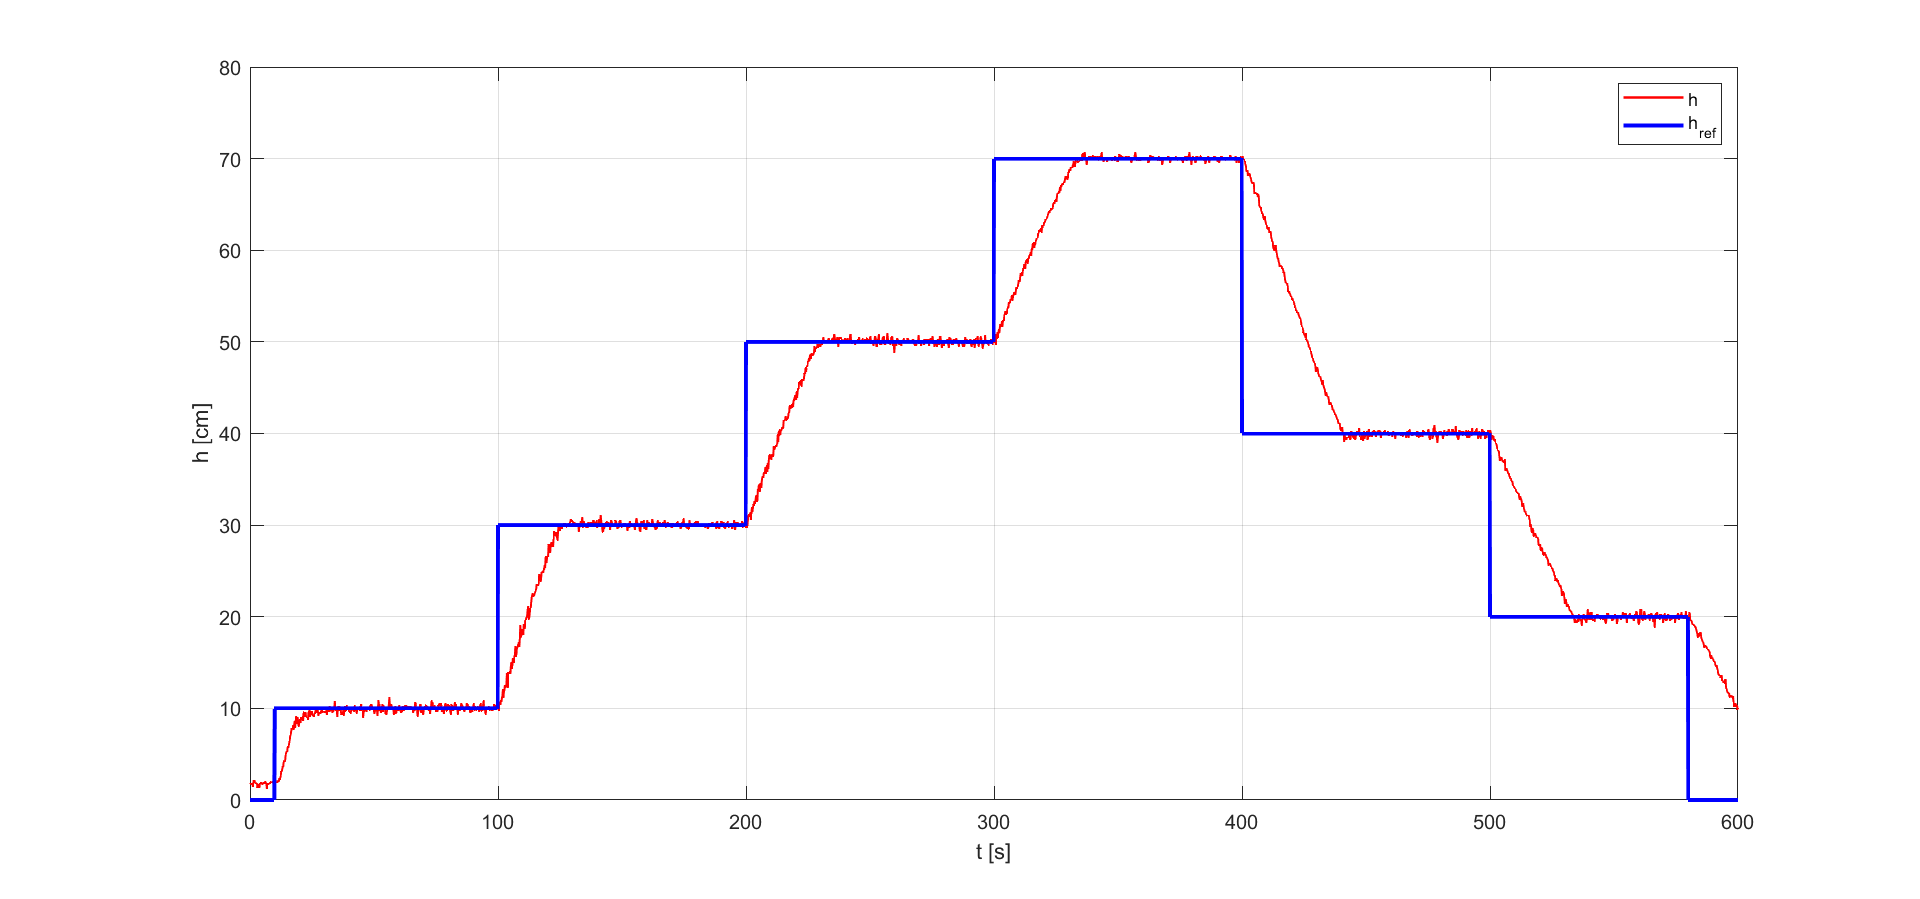
\includegraphics[width=\textwidth]{./include/meranie4.png}
	\end{center}
	\caption{Graf žiadanej a~meranej hodnoty výšky hladiny na~snímači v~štvrtom meraní [cm].}
	\label{fig:m4}
\end{figure}

\clearpage

\subsection{Meranie 5}
\label{sec:meranie5}

V piatom meraní sme si zvolili hodnoty. 
Výsledok simulácie môžeme vidieť na obrázku Obr.\ref{fig:m5}.
\begin{center}
\begin{tabular}{ |c|c| }
 \hline
 $K_p [-]$ & 50 \\
 $T_i [-]$ & 20 \\
 $T_d [-]$ & 0,1 \\
 \hline
\end{tabular}
\end{center}



\begin{figure}[!htbp]
	\begin{center}
		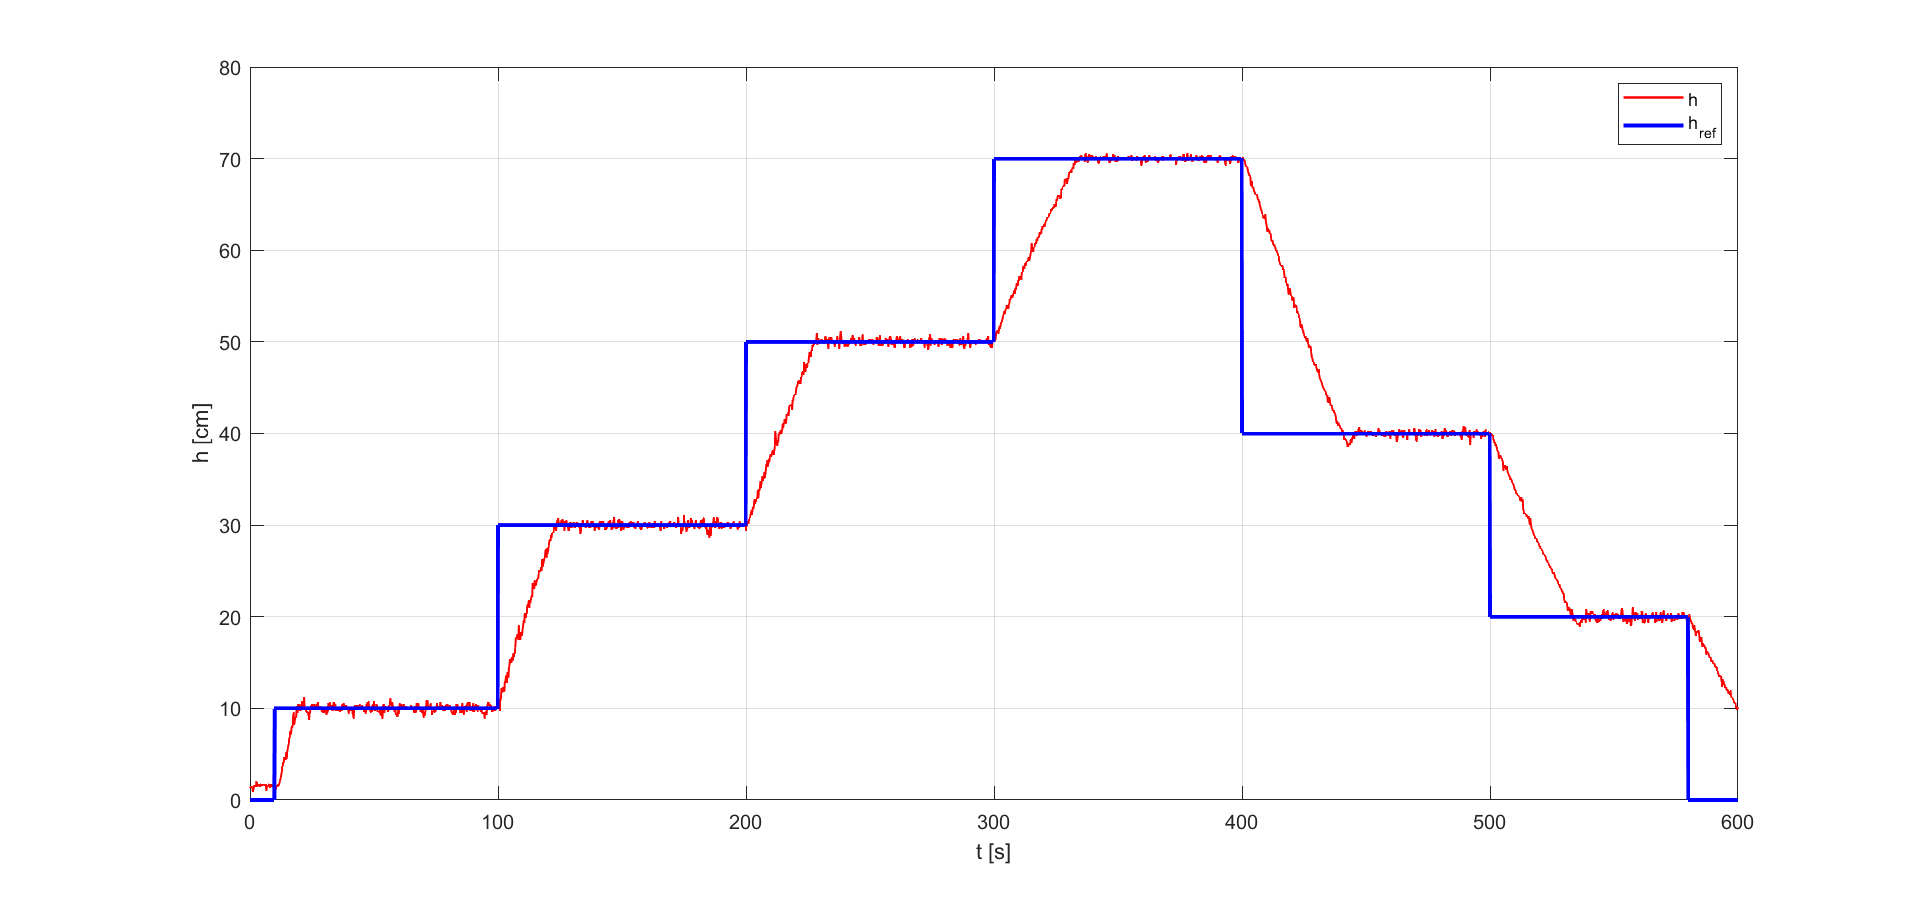
\includegraphics[width=\textwidth]{./include/meranie5.png}
	\end{center}
	\caption{Graf žiadanej a~meranej hodnoty výšky hladiny na~snímači v~piatom meraní [cm].}
	\label{fig:m5}
\end{figure}

\clearpage

\subsection{Meranie 6}
\label{sec:meranie6}

V šiestom meraní sme si zmenili hodnotu uzatvorenia výpustného ventilu zo 70\% na 50 \%, hodnoty
\textit{Kp}, \textit{Ti} a \textit{Td} sme ponechali rovnaké. Výsledok simulácie môžeme vidieť na Obr.~\ref{fig:m6}.

\begin{center}
\begin{tabular}{ |c|c| }
 \hline
 $K_p [-]$ & 50 \\
 $T_i [-]$ & 20 \\
 $T_d [-]$ & 0,1 \\
 \hline
 $Vstupny\_ventil[\%]$ & 100 \\
 $Vystupny\_ventil[\%]$ & 50 \\
 \hline
\end{tabular}
\end{center}

Výsledok simulácie môžeme vidieť na obrázkoch  .

\begin{figure}[!htbp]
	\begin{center}
		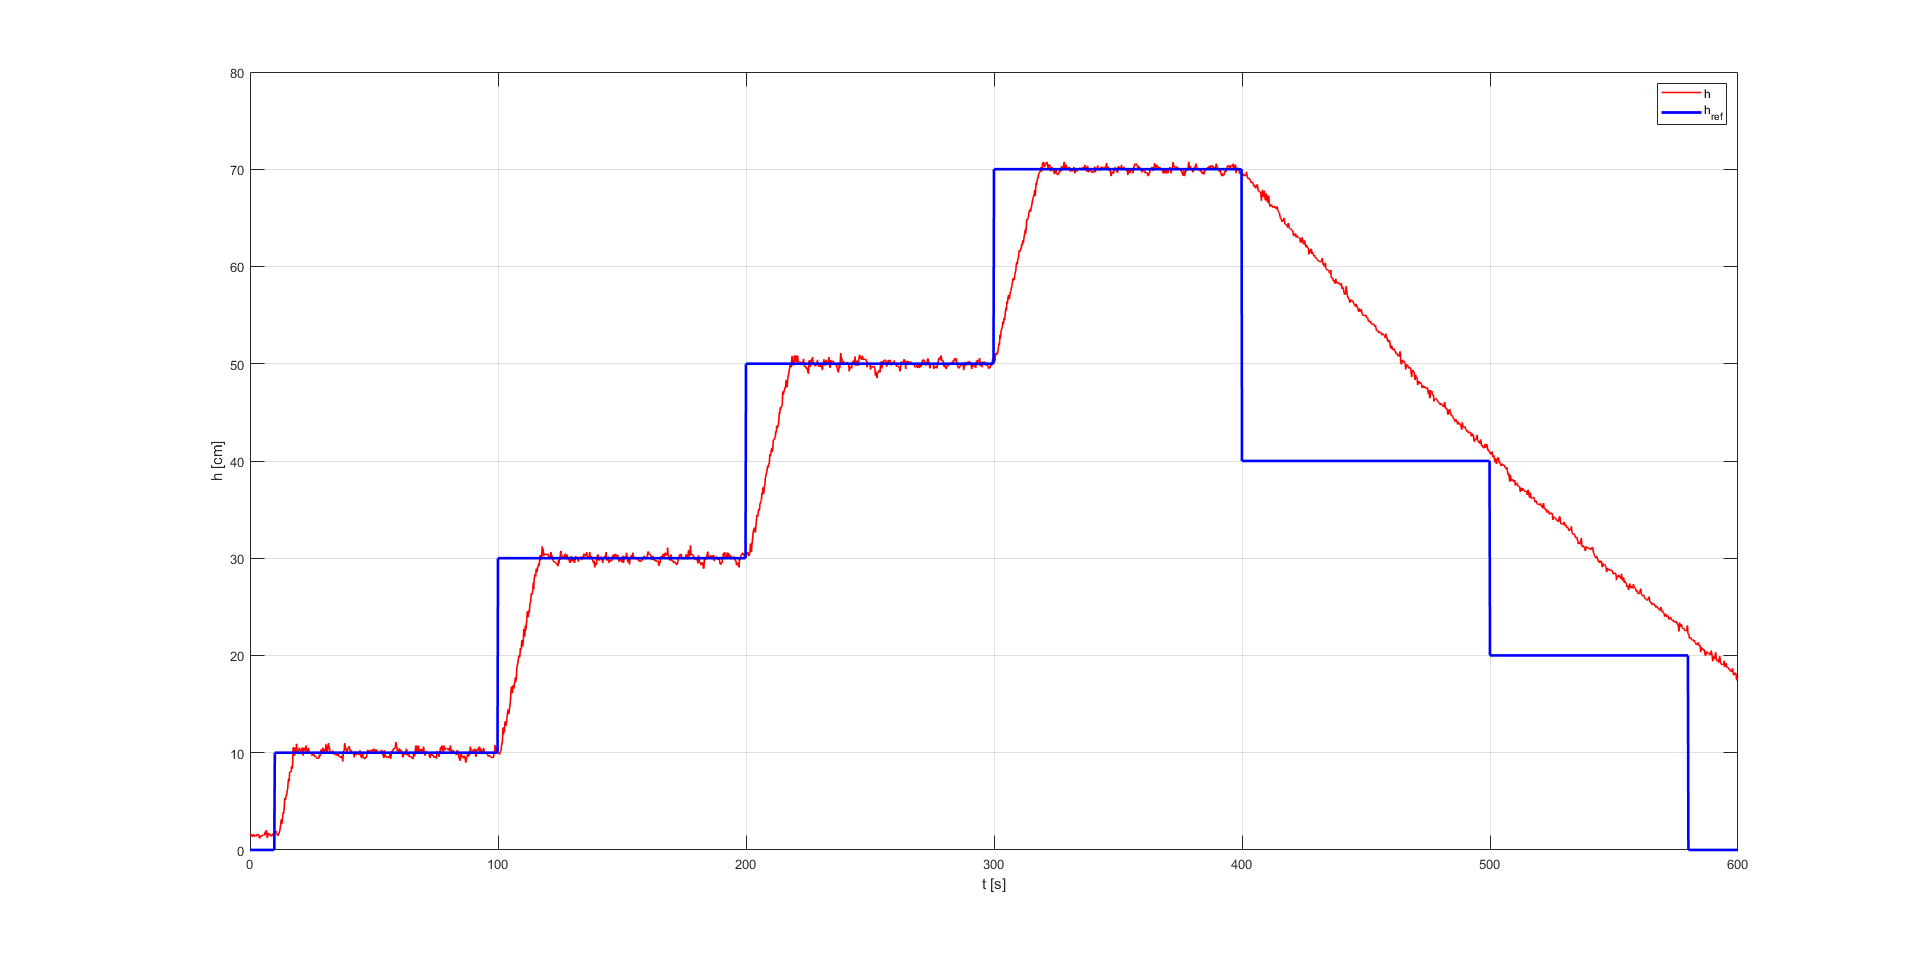
\includegraphics[width=\textwidth]{./include/meranie6.png}
	\end{center}
	\caption{Graf žiadanej a~meranej hodnoty výšky hladiny na~snímači v~šiestom meraní [cm].}
	\label{fig:m6}
\end{figure}

\clearpage

\subsection{Meranie 7}
\label{sec:meranie7}

V siedmom meraní sme si zmenili hodnotu uzatvorenia výpustného ventilu z 50\% na 80 \%, hodnoty
\textit{Kp}, \textit{Ti} a \textit{Td} sme ponechali rovnaké. Výsledok simulácie môžeme vidieť na Obr.~\ref{fig:m7}.

\begin{center}
\begin{tabular}{ |c|c| }
 \hline
 $K_p [-]$ & 50 \\
 $T_i [-]$ & 20 \\
 $T_d [-]$ & 0,1 \\
 \hline
 $Vstupny\_ventil[\%]$ & 100 \\
 $Vystupny\_ventil[\%]$ & 80 \\
 \hline
\end{tabular}
\end{center}


\begin{figure}[!htbp]
	\begin{center}
		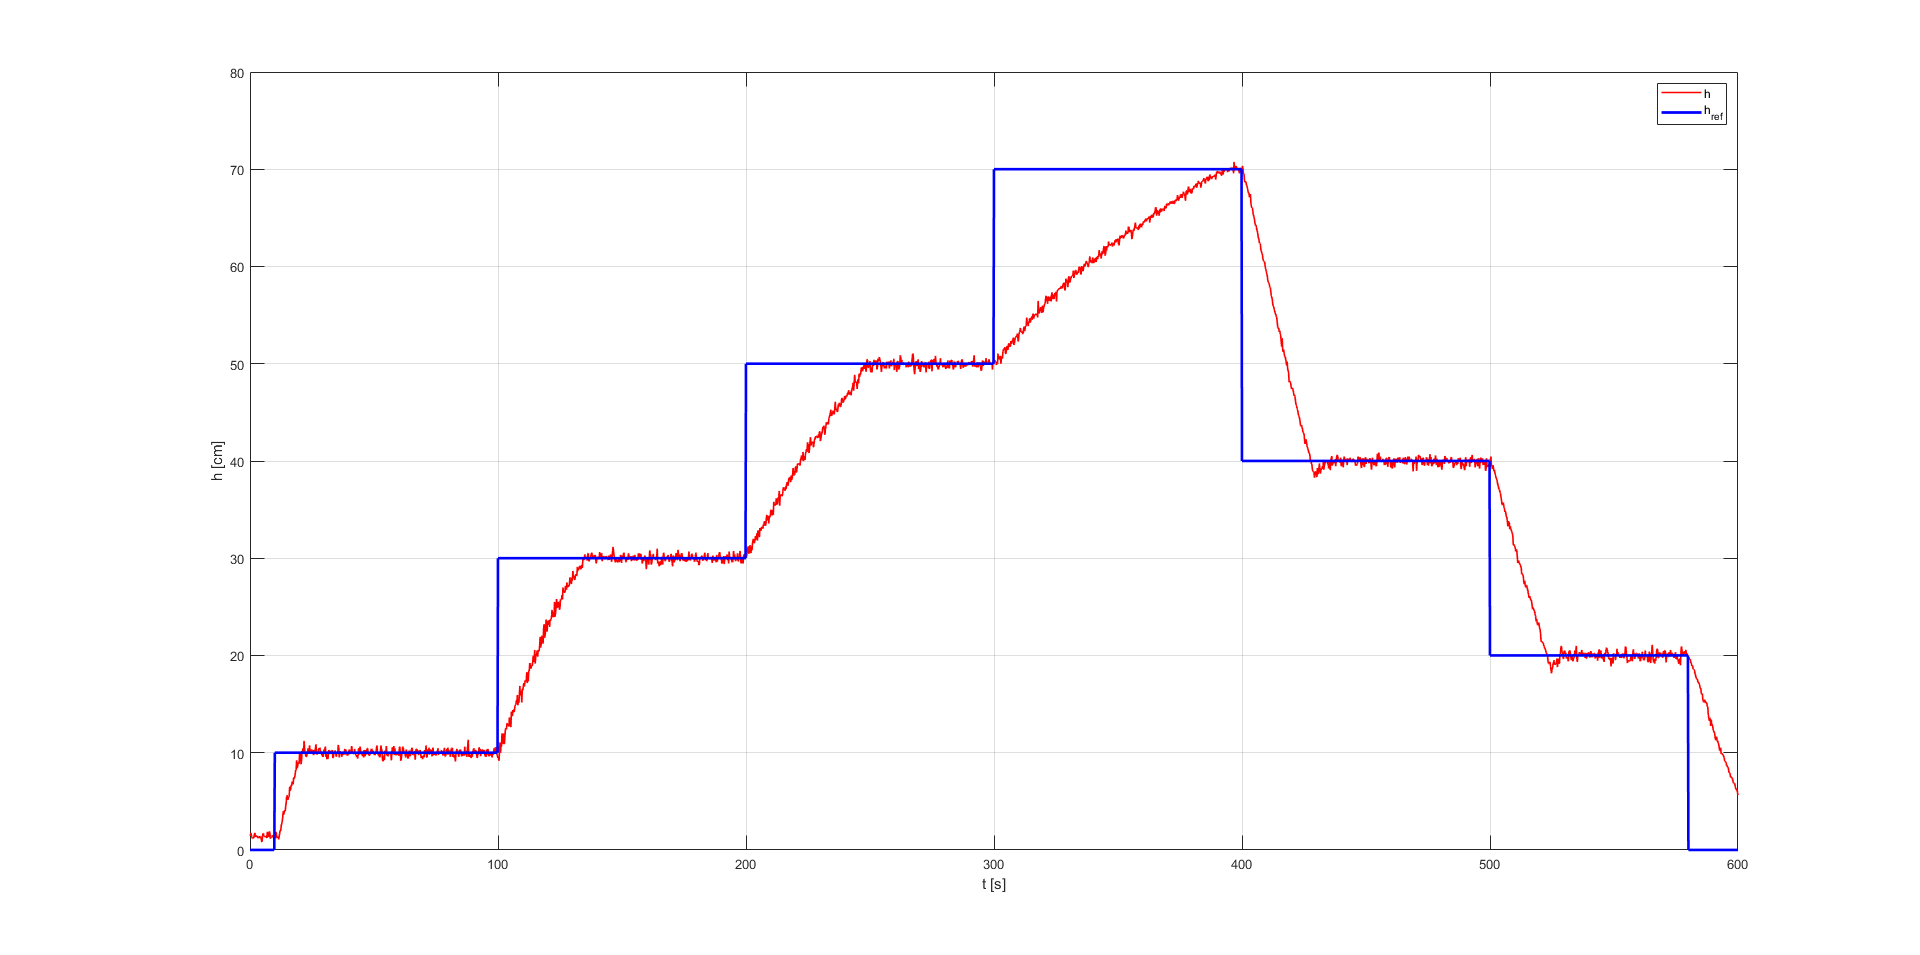
\includegraphics[width=\textwidth]{./include/meranie7.png}
	\end{center}
	\caption{Graf žiadanej a~meranej hodnoty výšky hladiny na~snímači v~siedmom meraní [cm].}
	\label{fig:m7}
\end{figure}


\clearpage

\section{Zhrnutie}
\label{sec:zhrnutie}

% V~tomto zadaní sme zisťovali dôsledok zmeny hodnoty hysterézy na~teplotu T2. Na~obrázkoch Obr.~\ref{fig:m1t2},
% Obr.~\ref{fig:m2t2}, Obr.~\ref{fig:m3t2} sme pozorovali nasledujúce správanie. Čím je hodnota hysterézy menšia,



\end{document}

